\documentclass[border=6pt]{standalone}
\usepackage{tikz}
\usetikzlibrary{arrows.meta,positioning,fit,calc}
\begin{document}
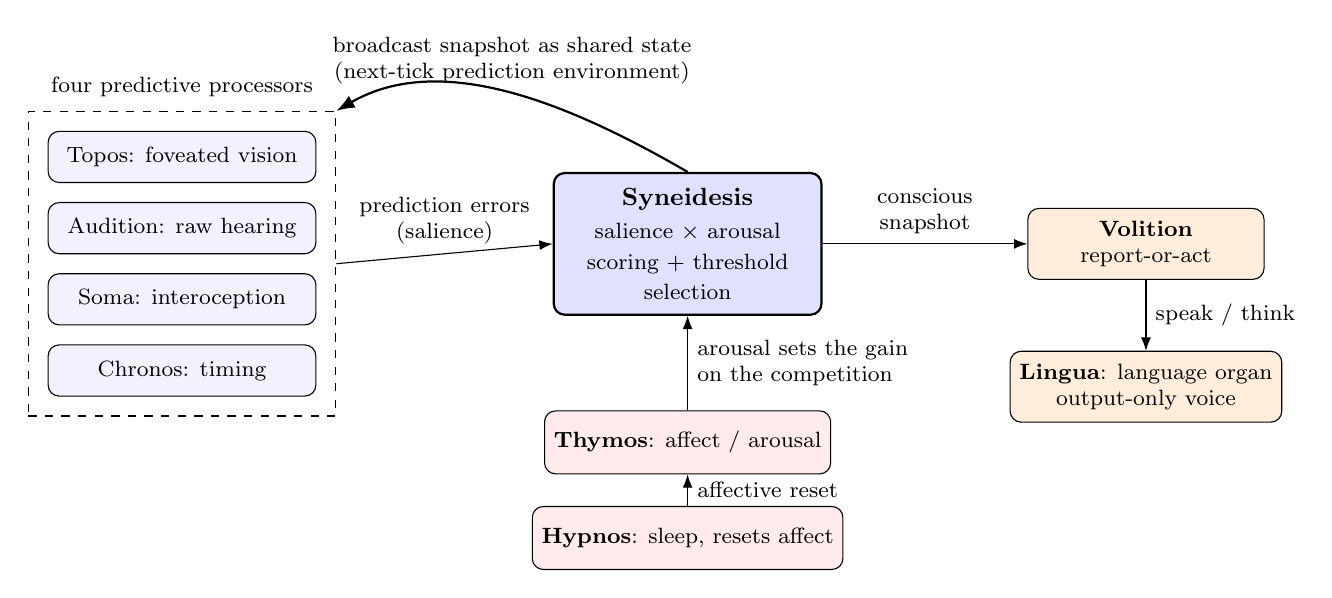
\begin{tikzpicture}[
  font=\small,>=Latex,
  mod/.style={draw, rounded corners, fill=blue!5, align=center, minimum width=34mm, minimum height=6.5mm, font=\footnotesize},
  aff/.style={draw, rounded corners, fill=red!8, align=center, minimum width=34mm, minimum height=8mm, font=\footnotesize},
  work/.style={draw, thick, rounded corners, fill=blue!12, align=center, minimum width=34mm, minimum height=18mm},
  act/.style={draw, rounded corners, fill=orange!14, align=center, minimum width=30mm, minimum height=9mm, font=\footnotesize},
]
% four predictive processors on the left
\node[mod] (m1) {Topos: foveated vision};
\node[mod, below=2.4mm of m1] (m2) {Audition: raw hearing};
\node[mod, below=2.4mm of m2] (m3) {Soma: interoception};
\node[mod, below=2.4mm of m3] (m4) {Chronos: timing};
\node[draw, dashed, fit=(m1)(m2)(m3)(m4), inner sep=7pt] (mods) {};
\node[font=\footnotesize, above=0.5mm of mods] {four predictive processors};
% workspace centre
\node[work, right=30mm of m2, yshift=-2mm] (syn) {\textbf{Syneidesis}\\[1pt]\footnotesize salience $\times$ arousal\\\footnotesize scoring $+$ threshold\\\footnotesize selection};
% affect below the workspace
\node[aff, below=12mm of syn] (aff) {\textbf{Thymos}: affect / arousal};
\node[aff, below=4mm of aff] (hyp) {\textbf{Hypnos}: sleep, resets affect};
% report-or-act and the language organ on the right
\node[act, right=26mm of syn] (vol) {\textbf{Volition}\\report-or-act};
\node[act, below=9mm of vol] (lin) {\textbf{Lingua}: language organ\\output-only voice};
% modules -> workspace (errors)
\draw[->] (mods.east) -- node[above, font=\footnotesize, align=center]{prediction errors\\(salience)} (syn.west);
% affect -> workspace (precision)
\draw[->] (aff) -- node[right, font=\footnotesize, align=left]{arousal sets the gain\\on the competition} (syn);
% hypnos -> thymos
\draw[->] (hyp) -- node[right, font=\footnotesize]{affective reset} (aff);
% broadcast loop back over the top
\draw[->, thick] (syn.north) to[out=150,in=30,looseness=0.9] node[above, font=\footnotesize, align=center]{broadcast snapshot as shared state\\(next-tick prediction environment)} (mods.north east);
% workspace -> volition
\draw[->] (syn) -- node[above, font=\footnotesize, align=center]{conscious\\snapshot} (vol);
% volition -> lingua
\draw[->] (vol) -- node[right, font=\footnotesize]{speak / think} (lin);
\end{tikzpicture}
\end{document}
